\documentclass[docid=CA07]{tcom_CA}
\begin{document}
\setcounter{section}{6}
\section{Challenge Activity 7 - Context Free Grammars}
\subsection{Exercise 1}%
{
\renewcommand{\thesubsubsection}{\thesubsection\alph{subsubsection}}
\subsubsection{Item a}
This CFG is ambiguous, because one can arrive at $\mathtt{if}\,(E)\,\mathtt{if}\,(E)\,S\,\mathtt{else}\,S$ using two different syntax trees.
\begin{center}
\begin{minipage}{0.45\textwidth}
	\begin{center}
		\begin{tikzpicture}
			\Tree 	[.S
						{$\mathtt{if}\,($}
						$E$
						$)$
						[.$S$
							{$\mathtt{if}\,($}
							$E$
							$)$
							$S$
							$\mathtt{else}$
							$S$
						]
					]
	  \end{tikzpicture}
	\end{center}
\end{minipage}%
\begin{minipage}{0.40\textwidth}
	\begin{center}
		\begin{tikzpicture}
			\Tree 	[.S
						{$\mathtt{if}\,($}
						$E$
						$)$
						[.$S$
							{$\mathtt{if}\,($}
							$E$
							$)$
							$S$
						]
						$\mathtt{else}$
						$S$
					]
	  \end{tikzpicture}
	\end{center}
\end{minipage}
\end{center}
\subsubsection{Item b}
It does not, given that for the example above the \texttt{else} can be associated to two different \texttt{if}'s through two different syntax trees.\\
Actually, the semantic of C-type if-else statements associates the \texttt{else} branch to the previous nearest \texttt{if} \textbf{that has not yet been matched}, given that processing starts on the left of the string.\\
To ensure that association, one can either adopt the C-style solution of adding curly brackets, which would result in the production rule
\begin{alignat*}{2}
	S \rightarrow \mathtt{if}\,(E)\,S\mid \mathtt{if}\,(E)\,\{S\}\,\mathtt{else}\,S\mid O
\end{alignat*}
or we can change the production rule that poses a problem, through one of two ways:
\begin{itemize}
	\item Eliminate the production that produces the problem, which yields
	\begin{alignat*}{2}
		S &\rightarrow \mathtt{if}\,(E)\,S\,\mathtt{else}\,S\mid O
	\end{alignat*}
	\item Change the origin of the problem, which is the first $S$ in the production rule $S \rightarrow \mathtt{if}\,(E)\,S\,\mathtt{else}\,S$ by limiting the expressions that can occur in that place:
	\begin{alignat*}{2}
		S &\rightarrow \mathtt{if}\,(E)\,S\mid \mathtt{if}\,(E)\,T\,\mathtt{else}\,S\mid O\\
		T &\rightarrow \mathtt{if}\,(E)\,T\mid E \mid  O 
	\end{alignat*}
\end{itemize}
The best option is probably the last one.
}
\end{document}
